\chapter{Extensions algorithmiques}
\label{chap:extensions}

Au-delà du sujet de base, le projet livre quatre extensions optionnelles. Toutes sont \textbf{opt-in} : leur activation se fait via un flag CLI ou une option CMake, et le chemin par défaut reste strictement inchangé en performance.

\section{Parallel attempts : K essais indépendants en parallèle}

\subsection{Motivation}

L'analyse du speedup OMP intra-attempt (Chapitre~\ref{chap:resultats}) révèle un plafonnement : au-delà de 8-16 threads, la parallélisation interne d'un seul attempt sature à cause des barrières BFS et de la contention atomique. Une approche complémentaire : au lieu de paralléliser \textit{dans} un attempt, lancer K attempts \textit{indépendants} en parallèle, chacun avec un seed dérivé différent.

\subsection{Algorithme}

\begin{algorithm}[H]
\caption{Parallel attempts orchestration}
\begin{algorithmic}[1]
\Require Options $opt$ avec $K = opt.\text{parallel\_attempts} > 1$
\For{batch\_start = 0, K, 2K, ... < $opt.\text{max\_attempts}$}
    \State $batch\_size \gets \min(K, opt.\text{max\_attempts} - batch\_start)$
    \State \textbf{parallel for} $k = 0$ \textbf{to} $batch\_size - 1$ \textbf{do}
        \State \quad $seed_k \gets \texttt{attempt\_seed}(opt.\text{seed}, batch\_start + k)$
        \State \quad $success_k \gets \texttt{serial\_run\_attempt}(waves_k, ...)$
    \State \textbf{end parallel for}
    \State $picked \gets$ premier $k$ tel que $success_k$
    \If{$picked \neq -1$}
        \State \Return $waves_{picked}$
    \EndIf
\EndFor
\State \Return échec
\end{algorithmic}
\end{algorithm}

\subsection{Garantie de déterminisme}

\begin{theorem}[Déterminisme parallel-attempts]
Pour un même seed initial, \texttt{parallel\_attempts=K} produit la même sortie qu'un retry séquentiel avec \texttt{max\_attempts=K}.
\end{theorem}

\begin{proof}
Le succès d'index minimum dans un batch $[0, K)$ est exactement le premier $k$ tel que $success_k$, qui est précisément le premier seed essayé par le retry séquentiel. Si tous échouent, on passe au batch suivant, qui correspond aux attempts $K \ldots 2K-1$, etc. CQFD.
\end{proof}

Vérifié par \texttt{test\_parallel\_attempts} : K=8 sur sample facile pointe \texttt{attempts == 1} (lowest-success), output bit-identique à un run séquentiel.

\subsection{Bypass du backend pour éviter l'oversubscription}

Chaque attempt parallèle utilise \texttt{serial\_run\_attempt} (de SolverCommon), \textbf{pas} le \texttt{propagate} du backend. Sinon, $K$ attempts × $T$ threads intra-attempt = $K \cdot T$ threads pour $T$ cores → catastrophe.

\subsection{Mesures}

Sur \texttt{terrain N=3 24×24}, total wallclock pour 4 seeds (Windows i9-10900K) :

\begin{table}[H]
\centering
\begin{tabular}{lrr}
\toprule
\textbf{Mode} & \textbf{Total} & \textbf{Speedup} \\
\midrule
sequential, 1 thread & 0.510 s & 1.0× \\
\texttt{--parallel-attempts 4 --threads 4} & 0.332 s & 1.54× \\
\texttt{--parallel-attempts 8 --threads 8} & 0.238 s & \textbf{2.14×} \\
\bottomrule
\end{tabular}
\caption{Parallel attempts : 2.14× wallclock sur workload à fort taux de retry.}
\label{tab:ext:parallel_attempts}
\end{table}

\subsection{Quand utiliser}

\begin{itemize}
    \item \textbf{Paie} sur les workloads à fort taux d'échec par attempt (terrain N=3 où ~10\% de succès par seed).
    \item \textbf{Inutile} sur les workloads qui réussissent du premier coup (binary\_5x5, smooth\_N3) : K attempts en parallèle = K× le travail pour le même résultat.
\end{itemize}

% =============================================================================
\section{Symétries D4 : expansion du tile set}
\label{sec:ext:symmetries}
% =============================================================================

\subsection{Motivation}

Le sujet et l'article de référence \cite{heaton2018wfc} mentionnent que le tile set peut être étendu par rotations / réflexions. Cette extension est utile sur des samples avec une orientation préférée (chemins, escaliers, branchages) : on veut que le motif s'applique uniformément dans toutes les orientations dans la sortie.

\subsection{Le groupe diédral $D_4$}

\begin{definition}[Groupe $D_4$]
Le groupe diédral d'ordre 8, $D_4$, est le groupe des symétries du carré : 4 rotations (0°, 90°, 180°, 270°) et 4 réflexions (axiales et diagonales).
\end{definition}

\begin{table}[H]
\centering
\begin{tabular}{cl}
\toprule
$S$ & Variantes générées par tuile \\
\midrule
1 & identité (défaut, comportement legacy) \\
2 & identité + rotation 180° \\
4 & 4 rotations \\
8 & 4 rotations + 4 réflexions ($D_4$ complet) \\
\bottomrule
\end{tabular}
\caption{Niveaux d'expansion D4 supportés par \texttt{TileSet::from\_sample(grid, N, S)}.}
\label{tab:ext:symmetries_levels}
\end{table}

\subsection{Implémentation}

\texttt{Tile::rotated\_90()} et \texttt{Tile::reflected\_horizontal()} sont des helpers purs qui retournent un nouveau \texttt{Tile}. Pour chaque pattern extrait, on génère ses variantes et on les déduplique par hash de contenu :

\begin{lstlisting}[language=C++]
template <typename Emit>
void emit_variants(const Tile& t, int symmetries,
                   std::unordered_map<Tile, int, TileHash>& seen,
                   Emit emit) {
    auto try_emit = [&](Tile&& v) {
        if (seen.find(v) != seen.end()) return;
        seen.emplace(v, 0);
        emit(std::move(v));
    };
    try_emit(Tile{t});
    if (symmetries == 1) return;
    Tile r90  = t.rotated_90();
    Tile r180 = r90.rotated_90();
    Tile r270 = r180.rotated_90();
    if (symmetries >= 2) try_emit(std::move(r180));
    if (symmetries >= 4) {
        try_emit(std::move(r90));
        try_emit(std::move(r270));
    }
    if (symmetries >= 8) {
        try_emit(t.reflected_horizontal());
        try_emit(t.rotated_90().reflected_horizontal());
        try_emit(r180.reflected_horizontal());
        try_emit(r270.reflected_horizontal());
    }
}
\end{lstlisting}

\subsection{Hot path inchangé à $S=1$}

À $S = 1$ (défaut), \texttt{from\_sample} suit exactement le code legacy :

\begin{lstlisting}[language=C++]
if (symmetries == 1) {
    auto [it, inserted] = index.try_emplace(...);
    // ... pas de génération de variantes, identique au legacy
} else {
    // ... expansion via emit_variants
}
\end{lstlisting}

Vérifié bit-à-bit par \texttt{test\_symmetries} : \texttt{from\_sample(g, N)} (legacy 2-args) produit le même TileSet que \texttt{from\_sample(g, N, 1)} (3-args explicite).

\subsection{Effet sur le tile set}

\begin{table}[H]
\centering
\begin{tabular}{lrrrr}
\toprule
\textbf{Sample} & \textbf{S=1} & \textbf{S=2} & \textbf{S=4} & \textbf{S=8} \\
\midrule
\texttt{skyline N=3} & 79 & 142 & 247 & 331 \\
\texttt{plant N=3} & 94 & 172 & 335 & 403 \\
\texttt{rooms N=3} & 14 & 14 & 14 & 14 \\
\bottomrule
\end{tabular}
\caption{Croissance du tile set selon $S$. Les patterns auto-symétriques (rooms binaire avec rotation/réflexion équivalentes) ne sont pas dupliqués.}
\label{tab:ext:tile_count}
\end{table}

L'auto-symétrie est gérée correctement : un sample uniformément peuplé de zéros, ou un damier, donne 1 tuile à $S = 1, 2, 4, 8$.

\subsection{Coût}

L'expansion se fait \textbf{une fois à l'extraction} (quelques µs même pour gros samples). Le solveur ne sait pas que les tuiles viennent de symétries, il voit juste un $L$ plus grand.

\textbf{Effet indirect} : $L'$ peut passer de 11 à 88 → bitsets parfois à 2 mots → solveur $\sim 1.5\times$ plus lent. Cohérent : plus de variantes = plus de choix par cellule.

% =============================================================================
\section{Backtracking avec snapshot delta-encodé}
\label{sec:ext:backtracking}
% =============================================================================

\subsection{Motivation}

Sur les samples très contraints (terrain N=3 sur petite grille), restart-on-contradiction épuise rapidement \texttt{max\_attempts} sans trouver de solution. Le backtracking, opt-in via \texttt{--backtrack}, explore l'arbre de recherche au lieu d'abandonner.

\subsection{Algorithme}

\begin{algorithm}[H]
\caption{Backtracking avec snapshot delta-encodé}
\begin{algorithmic}[1]
\State $stack \gets \emptyset$
\Loop
    \State $cell \gets \texttt{serial\_min\_entropy}()$
    \If{$cell < 0$}
        \State \Return succès
    \EndIf
    \State Ouvrir frame $F = \{cell, \text{candidates triés par fréquence desc}, \emptyset\}$
    \State Push $F$ sur $stack$
    \If{$\texttt{try\_top}(stack)$}
        \State Continue \Comment{forward}
    \EndIf
    \State $stack.\textsc{Pop}()$
    \While{$stack \neq \emptyset$}
        \State $\texttt{apply\_inverse}(stack.top.delta)$ \Comment{undo last try}
        \If{$\texttt{try\_top}(stack)$}
            \State Break \Comment{recovered}
        \EndIf
        \State $stack.\textsc{Pop}()$
    \EndWhile
    \If{$stack = \emptyset$}
        \State \Return échec
    \EndIf
\EndLoop
\end{algorithmic}
\end{algorithm}

\subsection{Optim 1 : Delta-encoded snapshot}

\begin{important}{Snapshot delta plutôt que snapshot complet}
Chaque frame ne stocke que les cellules effectivement modifiées par sa propagation. Mémoire : $\sim 50 \cdot W \cdot 16$ octets par frame (vs $r \cdot c \cdot W \cdot 8$ pour un snapshot plein), $\sim 80\times$ moins sur 64×64 binaire.
\end{important}

Implémentation : \texttt{serial\_propagate\_with\_delta} peek le pre-state en stack scratch, commit dans le delta uniquement si \texttt{and\_with} mute la cellule. Un flag \texttt{touched} évite le double-recording.

\begin{lstlisting}[language=C++]
struct WaveDelta {
    int words_per_cell = 0;
    std::vector<int> cells;
    std::vector<u64> before;
};

void apply_delta(Wave& wave, const WaveDelta& delta) {
    const int W = delta.words_per_cell;
    for (size_t k = 0; k < delta.cells.size(); ++k) {
        u64* dst = wave.raw_words() + delta.cells[k] * W;
        const u64* src = delta.before.data() + k * W;
        for (int w = 0; w < W; ++w) dst[w] = src[w];
    }
}
\end{lstlisting}

\subsection{Optim 2 : Composition avec parallel-attempts}

\texttt{solve\_parallel} détecte \texttt{use\_backtracking=true} et lance K recherches backtrack indépendantes, chacune avec un seed dérivé (donc ordre de tie-break différent → arbre d'exploration différent). Le succès d'index minimum gagne.

C'est la forme classique de \textit{parallel backtracking via independent searches} : pas de partage d'état entre recherches, pas de work stealing, donc simple et correct.

\subsection{Choix triés par fréquence descendante}

À chaque frame, les candidats sont triés par fréquence descendante : la tuile la plus probable est essayée en premier (heuristique « try the most likely »). Le backtracking est \textbf{déterministe} pour un seed donné, mais le seed influence l'ordre via \texttt{cell\_jitter} (entropy ties).

\subsection{Bypass du backend parallèle intra-attempt}

Le snapshot/restore n'a de sens qu'en single-threaded. Quand \texttt{use\_backtracking=true}, \texttt{solve\_sequential} invoque directement \texttt{serial\_run\_attempt\_backtrack} au lieu de la dispatch backend. Combiner backtrack + OMP intra-attempt ouvrirait des races inutilement complexes.

\subsection{Mesures}

\begin{table}[H]
\centering
\begin{tabular}{lrr}
\toprule
\textbf{Configuration} & \textbf{Temps} & \textbf{Résultat} \\
\midrule
\texttt{terrain N=3 32×32} retry-30 attempts & 0.38 s & \textbf{ÉCHEC} \\
\texttt{terrain N=3 32×32} \texttt{--backtrack} & 0.12 s & \textbf{succès} \\
\texttt{terrain N=3 32×32} \texttt{--parallel-attempts 8 --backtrack} & 0.20 s & succès \\
\bottomrule
\end{tabular}
\caption{Backtracking résout des instances où retry échoue. Le parallel-bt est plus lent ici car le single-bt trouve déjà vite (overhead K parallèle inutile sur ce cas).}
\label{tab:ext:backtrack}
\end{table}

% =============================================================================
\section{Démo Unreal Engine 5 : \texttt{wfc\_dungeon}}
\label{sec:ext:ue5}
% =============================================================================

\subsection{Motivation}

WFC est massivement utilisé pour la génération de niveaux dans les jeux. Pour démontrer que notre solveur s'intègre dans un pipeline réaliste, nous livrons une cible CLI \texttt{wfc\_dungeon} qui émet un JSON consommé par un plugin Unreal Engine 5.7.

\subsection{Pipeline}

\begin{figure}[H]
\centering
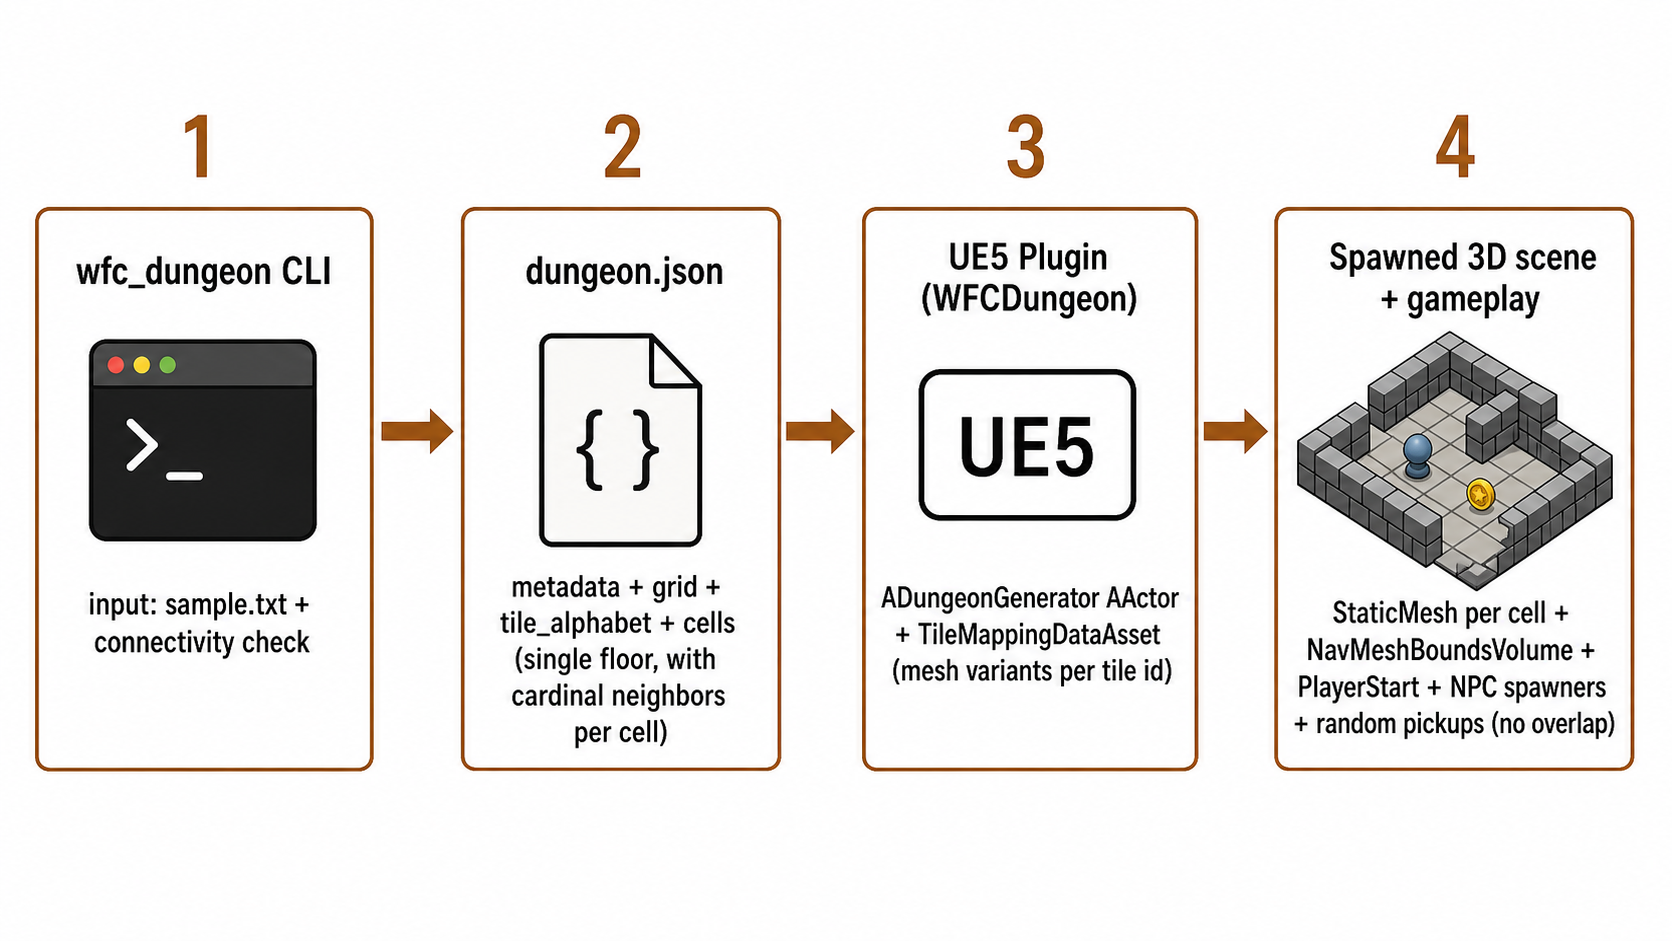
\includegraphics[width=0.95\linewidth]{results/figures/schemas/ue5_pipeline.png}
\caption{Pipeline asset → JSON → spawn de meshes UE5 + gameplay actors.}
\label{fig:ue5_pipeline}
\end{figure}

\subsection{Format JSON}

\begin{lstlisting}[language=C++]
{
  "version": 1,
  "metadata": { "sample": "...", "N": 2, "seed": 42 },
  "grid": { "rows": 24, "cols": 24, "cell_size_cm": 200,
            "wall_height_cm": 300 },
  "tile_alphabet": [ {"id": 0, "name": "floor"}, ... ],
  "cells": [
    { "row": 0, "col": 0, "tile_id": 0, "tile_name": "floor",
      "neighbors": { "n": 1, "s": 0, "e": 1, "w": 1 } },
    ...
  ]
}
\end{lstlisting}

Le pipeline est strictement \textbf{single-floor}. Une version
antérieure proposait un schéma v2 multi-étages avec auto-placement
d'escaliers ; le plugin UE5 a été simplifié pour coller au cas
mono-étage qui couvre les besoins de la démo, et le code mort
correspondant (flags \texttt{--levels}, \texttt{--floor-height},
\texttt{--stair-id}, struct \texttt{LevelGrid}, \texttt{place\_stairs},
branche multi-floor de \texttt{write\_dungeon\_json}) a été retiré.

\subsection{Connectivité par flood-fill BFS}

Avant d'émettre le JSON, \texttt{wfc\_dungeon} vérifie que les cellules
\textit{walkable} forment une composante connexe (flood-fill BFS). Si
plusieurs composantes sont détectées, l'algorithme re-roll avec un
nouveau seed (jusqu'à \texttt{--connectivity-attempts} fois). Garantit
qu'un joueur peut traverser tout le niveau.

\subsection{Plugin UE 5.7}

Le plugin \texttt{ue5\_plugin/WFCDungeon/} contient :

\begin{itemize}
    \item \texttt{UTileMappingDataAsset} : mappe chaque \texttt{tile\_id} vers un struct \{floor, wall, corner, door, plus arrays \texttt{*MeshVariants}\} + flags \texttt{bIsSolid}/\texttt{bIsDoor} + offset/scale. Les variants permettent un \textit{random pick} par tile id (fallback single-mesh).
    \item \texttt{ADungeonGenerator} : AActor qui parse le JSON, walk les cells, et spawne les \texttt{StaticMeshComponent} avec yaw cardinal (-90°N, +90°S, 0°E, 180°W).
\end{itemize}

\subsection{Gameplay actors et navmesh}

\texttt{ADungeonGenerator} expose des slots \texttt{TSubclassOf<AActor>}
pour transformer le dungeon en scaffold gameplay :

\begin{itemize}
    \item \texttt{PlayerStartClass} : 4 cellules walkable les plus proches du centre.
    \item \texttt{CornerSpawnerClass} (NPC) : scattered sur \texttt{NumCornerSpawners} cellules.
    \item \texttt{RandomPickupClass} : scattered sur \texttt{NumRandomPickups} cellules.
    \item Allocation non-collisionnelle : aucune cellule n'héberge deux catégories.
    \item Z-offsets dédiés (\texttt{GameplayActorZOffsetCm}, \texttt{PlayerStartZOffsetCm}) pour positionner les capsules au-dessus du sol.
\end{itemize}

\textbf{Volume de navigation auto-calculé} : un
\texttt{ANavMeshBoundsVolume} est spawné automatiquement, dimensionné
sur toute la grille via \texttt{UCubeBuilder} en éditeur (les polygones
de la brush sont reconstruits pour matcher visuellement le dungeon).
En runtime, fallback sur le scaling de l'actor.

\textbf{Bouton \textit{Generate Random}} : un appel
\textit{CallInEditor} qui spawn \texttt{wfc\_dungeon.exe} en
sous-processus avec un seed frais, écrit le JSON dans
\texttt{Saved/WFCTemp}, et chaîne le parsing immédiat. Une seule action
pour générer un nouveau dungeon.

\textbf{Périmètre fermé} : le flag \texttt{bWallOnBorders} (true par
défaut) ferme le pourtour du dungeon avec des walls, ce qui est utile
pour empêcher le joueur de sortir de la zone walkable.

\subsection{Build opt-in}

\texttt{-DBUILD\_DUNGEON=ON} active la cible \texttt{wfc\_dungeon}.
Sans, la cible n'est pas générée du tout (vérifié :
\texttt{ninja: no work to do} après reconfigure). Aucun impact sur le
benchmark, les ctests, ou les solveurs parallèles.

\subsection{Captures écran du dungeon généré}
\label{sec:ext:ue5:screens}

Trois captures du dungeon généré par \texttt{wfc\_dungeon} puis spawné dans
UE 5.7 par le plugin \texttt{ADungeonGenerator}. Le grid binaire
(\texttt{rooms.txt}, $N=2$, 24×24) est résolu par le solveur, sérialisé
en JSON, puis chaque cellule \textit{walkable} est instanciée comme
\texttt{StaticMeshComponent} (sol + variants) tandis que les cellules
\textit{solid} bordant un walkable spawnent un wall mesh avec yaw
cardinal correct.

\begin{figure}[H]
\centering
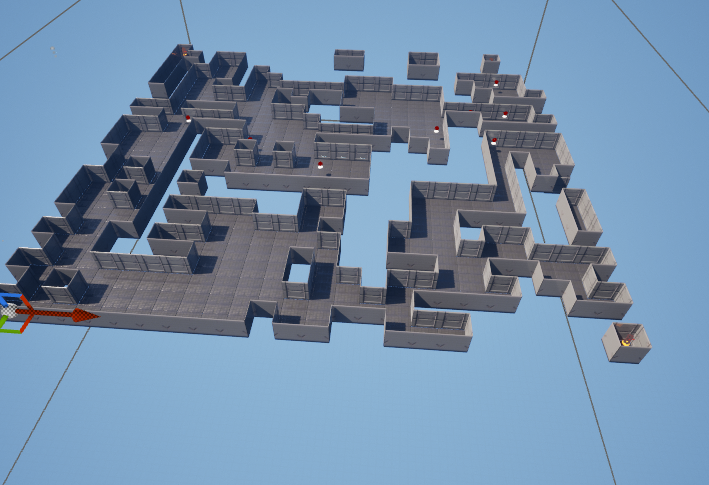
\includegraphics[width=0.95\linewidth]{results/figures/ue5/ue5_dungeon_01.png}
\caption{Vue d'ensemble du dungeon : grille 24×24 résolue par WFC,
spawnée en 3D avec sols texturés, walls, et périmètre fermé
(\texttt{bWallOnBorders=true}). Les pickups sont visibles sur
plusieurs cellules walkable.}
\label{fig:ue5_dungeon_01}
\end{figure}

\begin{figure}[H]
\centering
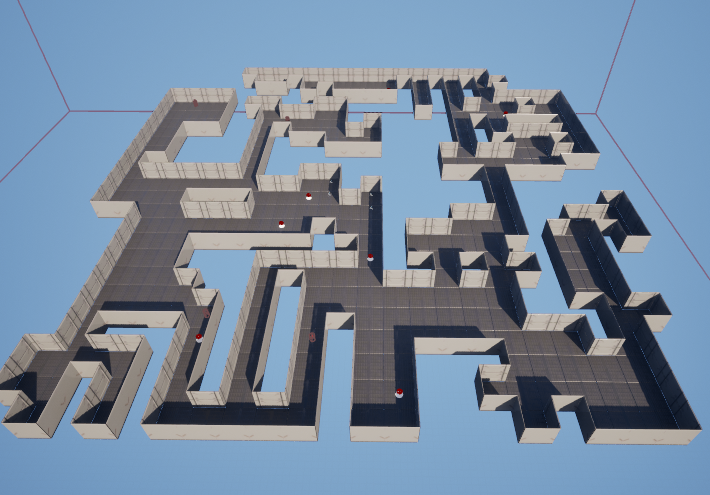
\includegraphics[width=0.95\linewidth]{results/figures/ue5/ue5_dungeon_02.png}
\caption[Détail d'une intersection de couloirs.]{Détail d'une
intersection de couloirs : les meshes de sol sont choisis
aléatoirement parmi \texttt{FloorMeshVariants} (variation visuelle),
les walls sont orientés selon leurs voisins walkable. La
connectivité globale walkable a été validée par flood-fill BFS
avant spawn.}
\label{fig:ue5_dungeon_02}
\end{figure}

\begin{figure}[H]
\centering
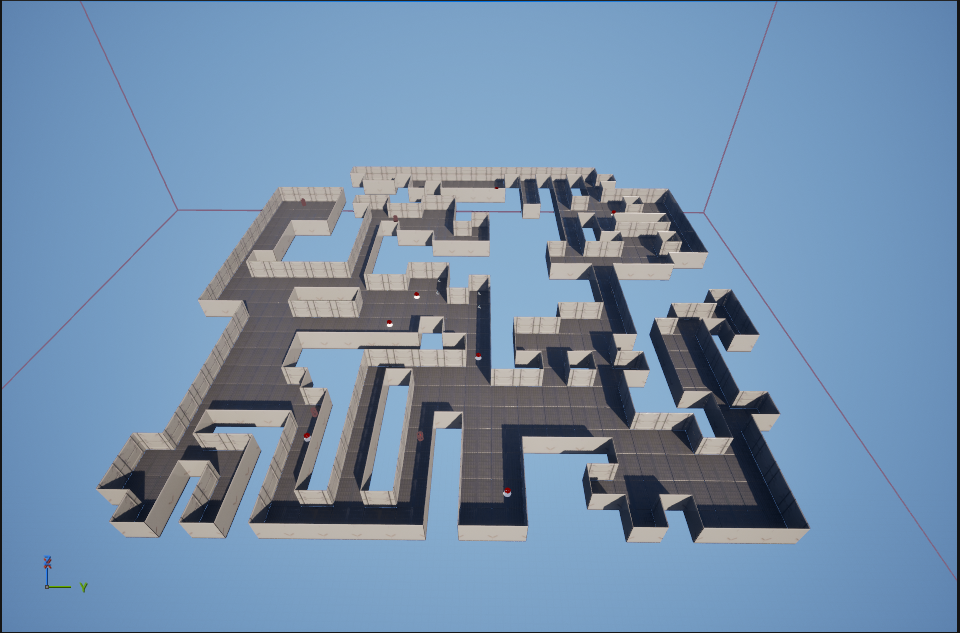
\includegraphics[width=0.95\linewidth]{results/figures/ue5/ue5_dungeon_03.png}
\caption[Vue d'une pièce avec PlayerStart, NPC et pickups.]{Vue
d'une pièce avec un \texttt{APlayerStart} (capsule), un NPC spawner
et plusieurs pickups. L'allocation non-collisionnelle garantit
qu'aucune cellule walkable n'héberge deux catégories d'actors. Le
\texttt{ANavMeshBoundsVolume} couvre toute la grille pour la
navigation IA.}
\label{fig:ue5_dungeon_03}
\end{figure}
